%%%%%%%%%%%%%%%%%%%%%%%%%%%%%%%%%%%%%%%%%%%%%%%%%%%%%%%%%%%%%%%%%%%%%%%%
\chapter{Ripasso di Termodinamica}
\label{cap:termodinamica}
%%%%%%%%%%%%%%%%%%%%%%%%%%%%%%%%%%%%%%%%%%%%%%%%%%%%%%%%%%%%%%%%%%%%%%%%

\begin{minipage}{0.35\textwidth}\end{minipage}\hfill
\begin{minipage}{0.65\textwidth}
\flushright{\em
If someone points out to you that your pet theory of the universe is in disagreement with Maxwell’s equations – then so much the worse for Maxwell’s equations. If it is found to be contradicted by observation – well, these experimentalists do bungle things sometimes. But if your theory is found to be against the second law of thermodynamics I can offer you no hope; there is nothing for it but to collapse in deepest humiliation.} % em
\vskip 0.25cm
\textsc{Sir A.S. Eddington}
\end{minipage}

%%%%%%%%%%%%%%%%%%%%%%%%%%%%%%%%%%%%%%%%%%%%%%%%%%%%%%%%%%%%%%%%%%%%%%%%
\section{Definizioni}
\label{sec1:def}
%%%%%%%%%%%%%%%%%%%%%%%%%%%%%%%%%%%%%%%%%%%%%%%%%%%%%%%%%%%%%%%%%%%%%%%%

La termodinamica si occupa sostanzialmente di trasformazioni di calore in lavoro e viceversa, ed è una branca della fisica prettamente {\em fenomenologica}; ciò in definitiva vale a dire che i principi fondamentali sui quali si basa sono assunti come postulati fondati sull'esperienza, e le conclusioni che se ne traggono sono in larghissima misura indipendenti dal dettaglio delle interazioni microscopiche tra i componenti elementari del sistema macroscopico in oggetto.

Dal punto di vista storico, lo studio dei fenomeni termodinamici ebbe nel 19-mo secolo, dal punto di vista delle ricadute tecnologiche, un'importanza difficile da sottovalutare: basti pensare che il motore a vapore fu determinante per la rivoluzione industriale. Occorre però considerare che la termodinamica non è nata, logicamente, dalle leggi del moto di Newton, ma su una base completamente empirica. Si può dire che siamo stati forzati a studiare la termodinamica perché abbiamo scoperto, sperimentalmente, che la Natura funziona in un certo modo, e non in un altro.

In meccanica (classica) generalmente si ha a che fare con punti materiali; specificare completamente lo stato di un sistema fisico al tempo $t$ significa assegnare tutte le posizioni e tutte le velocità (equivalentemente i momenti) delle $N$ ``particelle'' che compongono il sistema. Per un corpo macroscopico (per esempio, tipicamente, una mole di gas) lo stratosferico valore di $N$ rende improponibile questa procedura; se consideriamo poi che siamo interessati alle {\em proprietà medie} del sistema vediamo anche che la procedura è inutile. Occorre utilizzare quindi un nuovo concetto di {\em stato} di un sistema.

Prima di andare oltre occorre definire tre concetti: sistema macroscopico, grandezza estensiva e grandezza intensiva.

Interessarsi a un {\em sistema macroscopico} significa studiare il comportamento di un sistema formato da $N$ costituenti elementari (atomi, o molecole), confinato in un volume $V$, nel limite
\be
N \to \infty \quad\quad V \to \infty \quad\quad \textrm{con}\;\;n = N/V\;\; \textrm{fissato}.
\ee
Questo si chiama {\em limite termodinamico}; $n$ è la densità (numerica) di materia e $v = 1/n$ è il volume specifico.

Una grandezza è {\em intensiva} se nel limite termodinamico è una costante indipendente da $N$. È invece {\em estensiva} se nel limite termodinamico è lineare in $N$. Più precisamente
\bea
\lim_{N\to\infty} A &=& \textrm{costante} \quad\quad \textrm{se}\;\;A\;\;\textrm{è intensiva}; \nonumber\\
\lim_{N\to\infty} B/N &=& \textrm{costante} \quad\quad \textrm{se}\;\;B\;\;\textrm{è estensiva}.
\eea
Questi limiti si intendono indipendenti dalla forma del sistema, sotto la condizione che il rapporto superficie/volume non sia troppo grande; ciò in poche parole significa che la forma del contenitore deve essere regolare, non troppo strampalata.

In termodinamica si assume che una grandezza può essere intensiva o estensiva, ma non può avere un altro comportamento nel limite termodinamico. Questa in realtà è un'assunzione molto forte; limita in maniera sorprendente il tipo di interazioni microscopiche, tra i costituenti elementari del sistema, che possiamo prendere in considerazione. Per esempio, dobbiamo essere in grado di garantire che il sistema non collassi su sé stesso a causa di interazioni attrattive troppo forti, o che non esploda a causa di forze repulsive a grandi distanze.

Come vedremo in seguito (capitoli \ref{cap:canonico} e \ref{cap:grancanonico}) la presenza di un potenziale esterno modifica o può modificare la nostra intuizione relativa all'estensività di alcune grandezze termodinamiche.

%%%%%%%%%%%%%%%%%%%%%%%%%%%%%%%%%%%%%%%%%%%%%%%%%%%%%%%%%%%%%%%%%%%%%%%%
\subsection{Parametri termodinamici ed equilibrio}
\label{sec1:par}
%%%%%%%%%%%%%%%%%%%%%%%%%%%%%%%%%%%%%%%%%%%%%%%%%%%%%%%%%%%%%%%%%%%%%%%%

Introduciamo i {\em parametri termodinamici}: sono quantità macroscopiche misurabili come pressione $P$, volume $V$ e temperatura $T$, che trovano una definizione empirica (cioè sono quantità definite sperimentalmente tramite la procedura stessa con cui le si misura). Abbiamo in definitiva che lo {\em stato termodinamico} di un sistema macroscopico è specificato dall'insieme dei valori di tutti i parametri termodinamici necessari per una particolare descrizione del sistema in esame.

Quando lo stato termodinamico di un sistema non cambia nel tempo il sistema è detto essere in uno {\em stato di equilibrio termodinamico}. Generalmente (e sperimentalmente) si trova, per un sistema all'equilibrio i cui parametri siano $P$, $V$ e $T$, che questi tre parametri non sono indipendenti ma sono legati tra loro da una relazione funzionale del tipo
\be
\label{eq:stato_termo}
f(P,V,T) = 0
\ee
che è detta {\em equazione di stato}. Tale relazione fa sì che sia necessario specificare il valore di soli due parametri per individuare lo stato del sistema. L'equazione di stato definisce una superficie nello spazio tridimensionale $(P,V,T)$, e ogni punto su questa superficie rappresenta un possibile stato di equilibrio del sistema (vedi figura \ref{fig:eq-stato}).

%%%%%%%%%%%%%%%%%%%%%%%%%%%%%%%%%%%%%%%%%%%%%%%%%%%%%%%%%%%%%%%%%%%%%%%%
\begin{figure}[!ht]
  \centering
  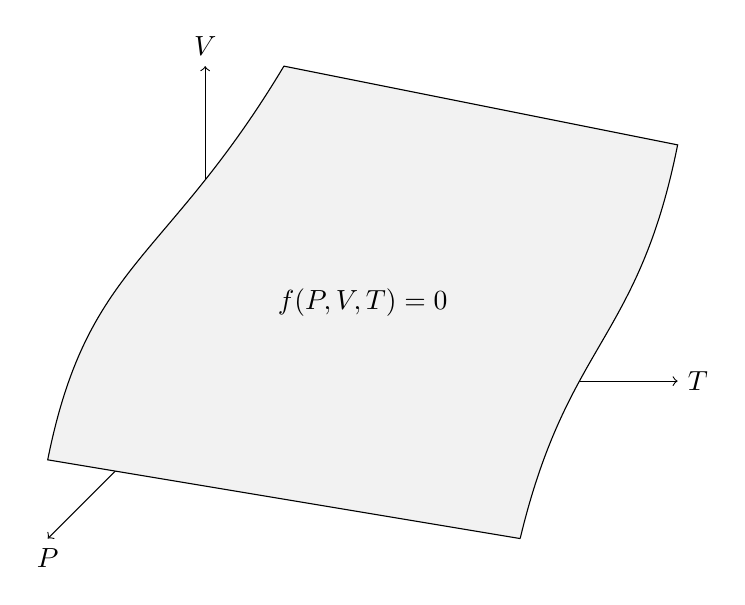
\begin{tikzpicture}[scale=1.0]
  \draw[->] (2,2)--(0,0) node[below=0.2]{$P$};
  \draw[->] (2,2)--(2,6) node[above=0.2]{$V$};  
  \draw[->] (2,2)--(8,2) node[right=0.2]{$T$};
  \draw[fill=gray!10!white] (6,0)--(0,1)..controls(0.5,3.5)and(1.5,3.5)..(3,6)
                                 --(8,5)..controls(7.5,2.5)and(6.6,2.5)..(6,0);
  \draw (4,3) node{$f(P,V,T) = 0$};
\end{tikzpicture}

  \caption{La superficie definita dall'equazione di stato nello spazio $(P,T,V)$.}
  \label{fig:eq-stato}
\end{figure}
%%%%%%%%%%%%%%%%%%%%%%%%%%%%%%%%%%%%%%%%%%%%%%%%%%%%%%%%%%%%%%%%%%%%%%%%

I cambiamenti di stato sono detti {\em trasformazioni termodinamiche}. Se le condizioni esterne che inducono il cambiamento di stato si modificano così lentamente che a ogni istante possiamo, con buona approssimazione, considerare il sistema in equilibrio, la trasformazione è detta {\em quasi--statica}. \`E detta invece {\em reversibile} se invertendo il  processo la trasformazione ripercorre all'indietro la sua storia, ossia il sistema torna allo stato da cui si era originariamente mosso, passando in direzione contraria per gli stati intermedi. Si ha che una trasformazione reversibile è necessariamente quasi--statica, ma non è vero il contrario: possiamo per esempio immaginare un gas che si espande molto lentamente e liberamente in elementi di volume infinitesimi successivi, e si vede subito che questa trasformazione è quasi--statica ma non reversibile.

Durante una trasformazione termodinamica il sistema può compiere del {\em lavoro}. Se il lavoro ha segno positivo ciò significa che è il sistema a compiere lavoro sull'ambiente esterno, mentre un segno negativo indica il contrario. A titolo di esempio consideriamo un gas contenuto in un recipiente cilindrico di area di base $S$, dotato a una sua estremità di un pistone mobile (vedi figura \ref{fig:pistone}). 

Sia $P$ la pressione che il gas esercita sulle pareti del contenitore; allora $PS$ è la forza esercitata dal gas sul pistone. Uno spostamento infinitesimo $\de{h}$ del pistone implica che si compie un lavoro infinitesimo (lavoro = forza $\times$ spostamento):
\be
\label{eq:lavoro_1}
\de{L} = PS\de{h}
\ee
(ricordare che lo spostamento è parallelo alla forza). Ma $S\de{h}$ è pari all'aumento di volume $\de{V}$ del sistema, così che si può scrivere
\be
\label{eq:lavoro_2}
\de{L} = P\de{V}
\ee
Sebbene questo risultato sia stato ottenuto in un caso particolare, ossia con una particolare geometria del contenitore, si può mostrare che esso è valido in generale, a patto che il rapporto tra superficie e volume del contenitore sia abbastanza piccolo.

Se la temperatura di un sistema aumenta senza che venga compiuto alcun lavoro, ciò significa che il sistema sta assorbendo {\em calore}. Il rapporto tra una quantità infinitesima $\de{Q}$ di calore e l'aumento infinitesimo $\de{T}$ di temperatura è chiamato {\em capacità termica} $C$ del sistema:
\be
\label{eq:cap_termica}
\de{Q} = C\de{T}
\ee
Sperimentalmente si trova che a parità di $\de{T}$, $\de{Q}$ cambia a seconda di come il sistema viene scaldato. In genere si considerano le capacità termiche $C_{V}$ (riscaldamento a volume costante) e $C_{P}$ (riscaldamento a pressione costante). La capacità termica per unità di massa (o per mole) è chiamata {\em calore specifico}.

%%%%%%%%%%%%%%%%%%%%%%%%%%%%%%%%%%%%%%%%%%%%%%%%%%%%%%%%%%%%%%%%%%%%%%%%
\subsection{Il gas ideale}
%%%%%%%%%%%%%%%%%%%%%%%%%%%%%%%%%%%%%%%%%%%%%%%%%%%%%%%%%%%%%%%%%%%%%%%%

%%%%%%%%%%%%%%%%%%%%%%%%%%%%%%%%%%%%%%%%%%%%%%%%%%%%%%%%%%%%%%%%%%%%%%%%
\begin{figure}[!ht]
\centering
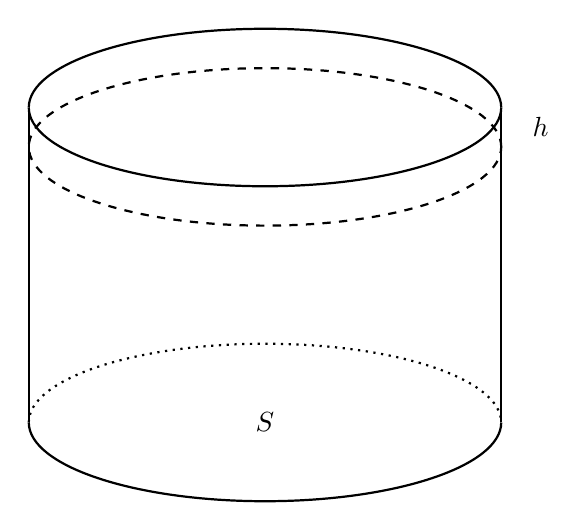
\begin{tikzpicture}[scale=1.0]
  \draw[thick] (0,0) arc[start angle=180, end angle=360, x radius=3, y radius=1];
  \draw[thick,dotted] (0,0) arc[start angle=180, end angle=0, x radius=3, y radius=1];
  \draw[thick] (0,0)--(0,4);
  \draw[thick] (6,0)--(6,4);
  \draw[thick] (0,4) arc[start angle=180, end angle=360, x radius=3, y radius=1];
  \draw[thick] (0,4) arc[start angle=180, end angle=0, x radius=3, y radius=1];
  \draw[thick,dashed] (6,3.5) arc[start angle=0, end angle=360, x radius=3, y radius=1];   
  \draw (6.5,3.75) node{$\de{h}$};
  \draw (3,0) node{$S$};
\end{tikzpicture}
\label{fig:pistone}
\caption{Dimostrazione, con una geometria particolare, che $L=P\de{V}$.}
\end{figure}
%%%%%%%%%%%%%%%%%%%%%%%%%%%%%%%%%%%%%%%%%%%%%%%%%%%%%%%%%%%%%%%%%%%%%%%%

Da un punto empirico si trova che tutti i gas, in condizioni di bassa densità, si comportano in maniera universale; il {\em gas ideale} è l'idealizzazione di tale comportamento limite. I parametri termodinamici di un gas  ideale classico sono la pressione $P$, il volume $V$, la temperatura $T$ e il numero di ``molecole'' $N$.

La prima cosa importante, riguardo il gas ideale (o {\em perfetto}), è che permette di definire una scala di {\em temperatura assoluta}. Si trova che gas diversi, mantenuti a una pressione costante molto bassa, forniscono indicazioni termometriche largamente indipendenti dalla natura del particolare gas utilizzato e indicano una temperatura $T$ proporzionale al volume occupato dal gas. L'unità della scala di misura per questa temperatura si prende, di solito, in modo tale che la differenza di temperatura tra il punto di ebollizione e il punto di congelamento dell'acqua alla pressione di $1$ atm risulti uguale a $100$. Come è ben noto, il punto di congelamento dell'acqua viene allora a corrispondere alla temperatura assoluta di $273.15$~K.

L'equazione di stato del gas ideale classico prende la forma:
\be
\label{eq:pvnkt}
PV = NkT
\ee
in cui $k$ è la costante di Boltzmann, il cui valore dipende dalla scelta convenzionale dell'unità di misura degli intervalli di temperatura. Per la scelta che abbiamo fatto prima (scala centigrada) si ha
\be
\label{eq:valk}
k \simeq 1.38 \times 10^{-23} \textrm{J/K}
\ee

%%%%%%%%%%%%%%%%%%%%%%%%%%%%%%%%%%%%%%%%%%%%%%%%%%%%%%%%%%%%%%%%%%%%%%%%
\section{Il primo principio della termodinamica}
\label{sec1:primo}
%%%%%%%%%%%%%%%%%%%%%%%%%%%%%%%%%%%%%%%%%%%%%%%%%%%%%%%%%%%%%%%%%%%%%%%%

Il primo principio della termodinamica esprime sostanzialmente la conservazione dell'energia in ambito termodinamico. Considerando un'arbitraria trasformazione termodinamica di un sistema, sia $\Delta Q$ la quantità netta di calore assorbita o ceduta dal sistema e $\Delta L$ il lavoro compiuto o subito dal sistema: la prima legge della termodinamica afferma che la quantità $\Delta U$, definita da
\be
\label{eq:DeltaU}
\Delta U = \Delta Q - \Delta L
\ee
è la stessa per tutte le trasformazioni che vanno da un dato stato iniziale a un dato stato finale. In altre parole, $\Delta U$ dipende solo dagli stati iniziali e finali del sistema, e non dal percorso fatto per arrivare allo stato finale dallo stato iniziale. Si vede subito che questo fatto unito alla possibilità di definire uno stato di riferimento $O$ per il quale si può porre $U_{O} = 0$ permette di definire una {funzione di stato} $U$, chiamata {\em energia interna}, definita a meno di una costante additiva arbitraria. Se $U$ è una funzione di stato, allora per una trasformazione infinitesima abbiamo che la quantità
\be
\label{eq:dU}
\de{U} = \de{Q} - \de{L}
\ee
è un differenziale esatto (mentre $\de{Q}$ e $\de{L}$ separatamente non lo sono). Se prendiamo $(P,V)$ come coppia di parametri indipendenti che definiscono lo stato di un sistema, avremo $U\equiv U(P,V)$ e anche, ovviamente,
\be
\label{eq:dU-PV}
\de{U} = \dparc{U}{P}{V}\de{P} + \dparc{U}{V}{P}\de{V}
\ee
La richiesta che $\de{U}$ sia un differenziale esatto si riduce alla proprietà secondo la quale l'ordine in cui vengono eseguite le derivate parziali non conta. Abbiamo quindi
\be
\label{eq:dU-PV-esatto}
\dparu{V}\left[\dparc{U}{P}{V}\right]_{P} = \dparu{P}\left[\dparc{U}{V}{P}\right]_{V}
\ee
Esprimendo $U$ prima in funzione della coppia $(V,T)$ e poi della coppia $(P,T)$ e considerando una trasformazione infinitesima reversibile (in cui $\de{L} = P\de{V}$) si ottengono facilmente le relazioni.
\bea
\label{eq:cvcp}
C_{V} &\equiv \left(\frac{\Delta Q}{\Delta T}\right)_{V} = \dparc{U}{T}{V}\nonumber\\
C_{P} &\equiv \left(\frac{\Delta Q}{\Delta T}\right)_{P} = \dparc{H}{T}{P} 
\eea
in cui $H = U + PV$ è detta {\em entalpia} del sistema; vedi esercizio (\ref{ex1:cvcp1}).

\subsection{Espansione libera di un gas ideale}
%%%%%%%%%%%%%%%%%%%%%%%%%%%%%%%%%%%%%%%%%%%%%%%%%%%%%%%%%%%%%%%%%%%%%%
\begin{figure}[!ht]
  \centering
  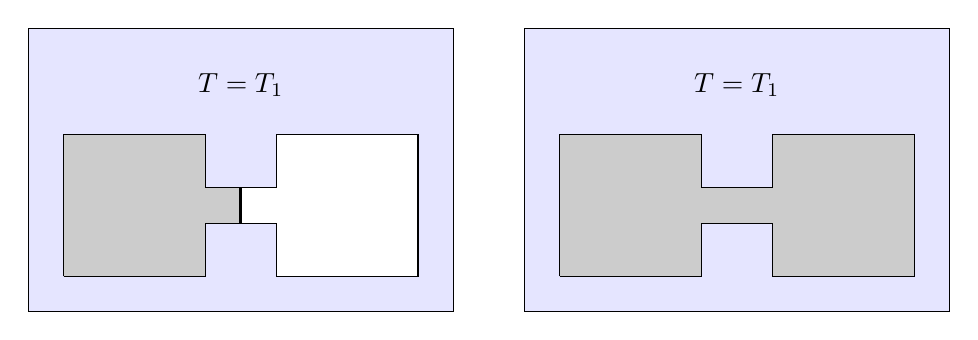
\begin{tikzpicture}[scale=0.9]
  \draw[fill=blue!10!white] (0,0)--(0,4)--(6,4)--(6,0)--(0,0);
  \draw[fill=white]      
        (0.5,0.5)--(0.5,2.5)--(2.5,2.5)--(2.5,1.75)--(3.5,1.75)--(3.5,2.5)--(5.5,2.5)--
        (5.5,0.5)--(3.5,0.5)--(3.5,1.25)--(2.5,1.25)--(2.5,0.5)--(0.5,0.5);
  \draw[fill=gray!40!white]      
        (0.5,0.5)--(0.5,2.5)--(2.5,2.5)--(2.5,1.75)--(3.0,1.75)--(3.0,1.25)--(2.5,1.25)--
        (2.5,0.5)--(0.5,0.5);
  \draw[very thick] (3.0,1.75)--(3.0,1.25);
  \draw (3,3.2) node{$T = T_1$};  
 
  \draw[fill=blue!10!white,xshift=7cm] (0,0)--(0,4)--(6,4)--(6,0)--(0,0);
  \draw[fill=gray!40!white,xshift=7cm]      
        (0.5,0.5)--(0.5,2.5)--(2.5,2.5)--(2.5,1.75)--(3.5,1.75)--(3.5,2.5)--(5.5,2.5)--
        (5.5,0.5)--(3.5,0.5)--(3.5,1.25)--(2.5,1.25)--(2.5,0.5)--(0.5,0.5);
  \draw (3,3.2) [xshift=7cm] node{$T = T_1$};  
\end{tikzpicture}

  \caption{Espansione libera di un gas perfetto.}
  \label{fig:espansione}
\end{figure}
%%%%%%%%%%%%%%%%%%%%%%%%%%%%%%%%%%%%%%%%%%%%%%%%%%%%%%%%%%%%%%%%%%%%%%
Si consideri l'espansione libera, nel vuoto, di un gas ideale (vedi figura \ref{fig:espansione}). Sperimentalmente si trova $T_{2} = T_{1}$. Poiché il gas non compie lavoro, abbiamo anche $\Delta L = 0$, e dal fatto che $\Delta T = 0$ ricaviamo subito $\Delta Q = 0$, e quindi in definitiva $\Delta U = 0$.

Poiché nulla ci impedisce di assumere che $U$ sia funzione di $T$ e $V$, dal risultato sopra ricaviamo immediatamente che l'energia interna di un gas ideale dipende solo dalla temperatura. Va notato che questo risultato può essere ricavato per via puramente teorica usando la seconda legge della termodinamica; per un punto di vista leggermente diverso, vedi l'esercizio (\ref{ex1:PVNkT}).

%%%%%%%%%%%%%%%%%%%%%%%%%%%%%%%%%%%%%%%%%%%%%%%%%%%%%%%%%%%%%%%%%%%%%%
\subsection{Energia interna}
%%%%%%%%%%%%%%%%%%%%%%%%%%%%%%%%%%%%%%%%%%%%%%%%%%%%%%%%%%%%%%%%%%%%%%
Visto che $U$ dipende solo da $T$, possiamo scrivere
\be
C_{V} = \dparc{U}{T}{V} = \dtot{U}{T}
\ee
Assumendo che $C_{V}$ sia indipendente dalla temperatura, otteniamo 
\be
U = C_{V}T + \textrm{costante}
\ee
e la costante additiva può essere posta arbitrariamente a zero, visto che $U$ stessa è definita a meno di una costante additiva arbitraria.

%%%%%%%%%%%%%%%%%%%%%%%%%%%%%%%%%%%%%%%%%%%%%%%%%%%%%%%%%%%%%%%%%%%%%%
\subsection{Calori specifici}
%%%%%%%%%%%%%%%%%%%%%%%%%%%%%%%%%%%%%%%%%%%%%%%%%%%%%%%%%%%%%%%%%%%%%%
Per un gas ideale (con un numero fissato $N$ di particelle) troviamo subito che l'entalpia è funzione della sola temperatura:
\be
H = U + PV = (C_{V} + Nk)T
\ee
e troviamo quindi
\be
C_{P} = \dparc{H}{T}{P} = \dtot{H}{T} = C_{V} + Nk
\ee
ovvero
\be
\label{eq:diff-cs}
C_{P} - C_{V} = Nk
\ee
L'ultimo risultato può essere interpretato nel senso che è più efficiente fornire calore a un gas ideale tenendo costante il volume piuttosto che la pressione. Intuitivamente ciò è dovuto al fatto che a volume costante non viene compiuto alcun lavoro, in modo tale che tutta l'energia fornita dal calore va ad aumentare l'energia interna. Usando la teoria cinetica si può far vedere che
\bea
\label{eq:cv-mono-bi}
C_{V} &=& \frac{3}{2} Nk\qquad\mbox{per un gas monoatomico}\\
C_{V} &=& \frac{5}{2} Nk\qquad\mbox{per un gas biatomico}\\
\eea

%%%%%%%%%%%%%%%%%%%%%%%%%%%%%%%%%%%%%%%%%%%%%%%%%%%%%%%%%%%%%%%%%%%%%%
\subsection{Trasformazioni adiabatiche}
%%%%%%%%%%%%%%%%%%%%%%%%%%%%%%%%%%%%%%%%%%%%%%%%%%%%%%%%%%%%%%%%%%%%%%

Se il sistema fisico in esame è sottoposto a una trasformazione reversibile senza scambio di calore con l'esterno, allora la trasformazione si chiama {\em adiabatica}. In questo caso si ha $\de{Q} = 0$ e l'equazione che esprime il primo principio può essere scritta come
\be
\label{eq:adiabatica-uno}
C_{V}\de{T} + P\de{V} = 0 
\ee
e usando $P = NkT/V$ otteniamo
\be
C_{V}\de{T} + \frac{NkT}{V}\de{V} = 0 
\ee
ossia
\be
\frac{\de{T}}{T} + \frac{Nk}{C_{V}}\frac{\de{V}}{V} = 0 
\ee
Integrando otteniamo
\be
\label{eq:adiabatica-due}
TV^{\gamma-1} = \textrm{costante} 
\ee
in cui abbiamo introdotto $\gamma = C_{P}/C_{V}$, e usando l'equazione di stato otteniamo
\be
\label{eq:adiabatica-tre}
PV^{\gamma} = \textrm{costante} 
\ee

%%%%%%%%%%%%%%%%%%%%%%%%%%%%%%%%%%%%%%%%%%%%%%%%%%%%%%%%%%%%%%%%%%%%%%
\section{Il secondo principio della termodinamica}
\label{sec1:secondo}
%%%%%%%%%%%%%%%%%%%%%%%%%%%%%%%%%%%%%%%%%%%%%%%%%%%%%%%%%%%%%%%%%%%%%%

Il secondo principio della termodinamica stabilisce delle limitazioni ben precise sulla possibilità di trasformare calore in lavoro ed esclude la possibilità di costruire una macchina a moto perpetuo di seconda specie. Il secondo principio può essere esposto o con l'enunciato di Lord Kelvin o con l'enunciato di Clausius. 

{\em Enunciato di Lord Kelvin}: è impossibile realizzare una trasformazione termodinamica il cui unico risultato sia una trasformazione in lavoro di calore tratto da una sorgente a temperatura uniforme.

{\em Enunciato di Clausius}: è impossibile realizzare una trasformazione termodinamica il cui unico risultato sia il passaggio di calore da un corpo a una data temperatura a un altro a temperatura più alta.

%%%%%%%%%%%%%%%%%%%%%%%%%%%%%%%%%%%%%%%%%%%%%%%%%%%%%%%%%%%%%%%%%%%%%%
\subsection{Il ciclo di Carnot}
%%%%%%%%%%%%%%%%%%%%%%%%%%%%%%%%%%%%%%%%%%%%%%%%%%%%%%%%%%%%%%%%%%%%%%

Si consideri la trasformazione termodinamica reversibile ciclica raffigurata in figura \ref{fig:carnot}. I rami $AB$ e $CD$ rappresentano isoterme (il primo a temperatura costante $T_{2}$ e il secondo a temperatura costante $T_{1}$), mentre i rami $BC$ e $DA$ adiabatiche. Tale trasformazione prende il nome di {\em ciclo di Carnot}, e un motore che compia effettivamente il ciclo si chiama {\em macchina di Carnot}.

In un ciclo di Carnot, la variazione di energia interna è nulla: ciò significa che il lavoro totale compiuto dalla macchina sarà pari alla quantità di calore scambiata con l'esterno. Lungo le adiabatiche lo scambio di calore è nullo; invece, lungo l'isoterma $AB$ il motore assorbe una quantità di calore pari a $Q_{2}$, mentre lungo l'isoterma $CD$ cede una quantità di calore pari a $Q_{1}$. Abbiamo quindi
%
\be
\label{eq:lavoro-carnot}
L = Q_{2} - Q_{1}
\ee
%
Il rendimento $\eta$ di una macchina di Carnot è definito da
%
\be
\label{eq:etaQ}
\eta = \frac{L}{Q2} = \frac{Q_{2}-Q_{1}}{Q_{2}} = 1 - \frac{Q_{1}}{Q_{2}}
\ee
%
%%%%%%%%%%%%%%%%%%%%%%%%%%%%%%%%%%%%%%%%%%%%%%%%%%%%%%%%%%%%%%%%%%%%%%
\begin{figure}[!ht]
	\centering
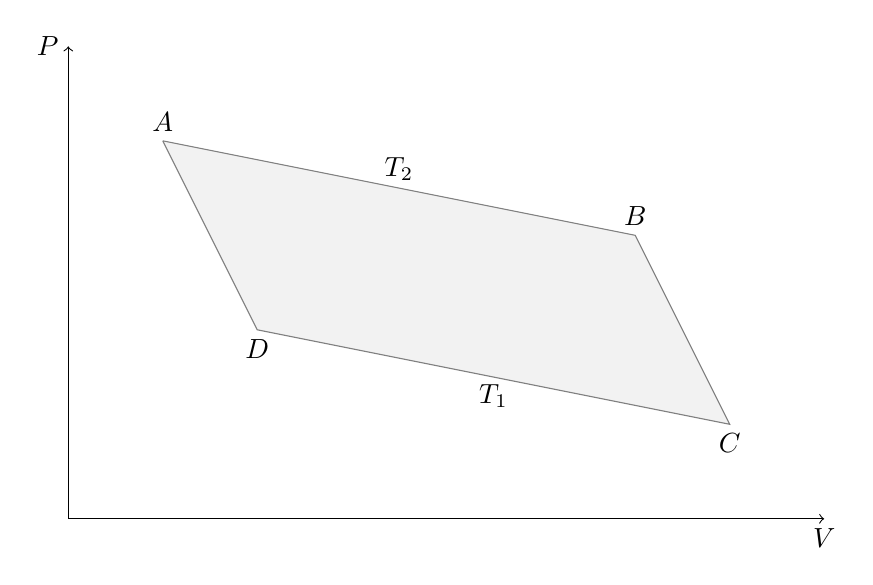
\begin{tikzpicture}[scale=1.2]
  \draw[->] (0,0)--(8,0) node[anchor=north] {$V$};
  \draw[->] (0,0)--(0,5) node[anchor=east] {$P$};
  \draw[gray,fill=gray!10!white] (1,4)--(6,3)--(7,1)--(2,2)--(1,4);
  \draw (1,4.2) node{$A$};
  \draw (6,3.2) node{$B$};
  \draw (7,0.8) node{$C$};
  \draw (2,1.8) node{$D$};
  \draw (3.5,3.7) node{$T_2$};
  \draw (4.5,1.3) node{$T_1$};
\end{tikzpicture}
	\caption{Rappresentazione schematica e semplificata del ciclo di Carnot, in cui le isoterme e le adiabatiche sono rappresentate come rette. Si veda il testo per la spiegazione dei simboli. L'area tratteggiata è il lavoro compiuto dal ciclo.}
	\label{fig:carnot}
\end{figure}
%%%%%%%%%%%%%%%%%%%%%%%%%%%%%%%%%%%%%%%%%%%%%%%%%%%%%%%%%%%%%%%%%%%%%%
Si può dimostrare che tutti i motori termici reversibili che operano tra le temperature $T_{2}$ e $T_{1}$ (con $T_{2}>T_{1}$) hanno lo stesso rendimento del motore di Carnot, mentre i motori irreversibili hanno rendimenti che non sono mai maggiori di quelli dei motori reversibili. Ciò significa che il rapporto $Q_{2}/Q_{1}$ è universale, e non dipende dai dettagli del motore in esame, ma dipende solo dalle temperature $T_{2}$ e $T_{1}$, e questo fatto, come vediamo subito, permette di definire una temperatura termodinamica assoluta. Possiamo infatti scrivere
\be
\frac{Q_{2}}{Q_{1}} = f(T_{1}, T_{2})
\ee
e inoltre si può dimostrare che
\be
\label{eq:ft1t2}
f(T_{1}, T_{2}) = \frac{\theta(T_{2})}{\theta(T_{1})}
\ee
in cui $\theta(T)$ è una certa funzione della temperatura, definita a meno di una costante moltiplicativa arbitraria. Usando la scala definita dal grado centigrado si può dimostrare che $\theta(T)$ coincide con la temperatura assoluta introdotta per i gas perfetti. Abbiamo quindi, in definitiva,
\be
\frac{Q_{2}}{Q_{1}} = \frac{T_{2}}{T_{1}}
\ee
e possiamo riscrivere il rendimento come
\be
\eta = 1 - \frac{T_{1}}{T_{2}}
\ee

%%%%%%%%%%%%%%%%%%%%%%%%%%%%%%%%%%%%%%%%%%%%%%%%%%%%%%%%%%%%%%%%%%%%%%
\section{L'entropia termodinamica}
\label{sec1:entropia}
%%%%%%%%%%%%%%%%%%%%%%%%%%%%%%%%%%%%%%%%%%%%%%%%%%%%%%%%%%%%%%%%%%%%%%

Il secondo principio della termodinamica ci permette di definire una nuova funzione di stato: l'entropia termodinamica. Cominciamo enunciando il teorema seguente, la cui dimostrazione può essere trovata su qualsiasi testo di termodinamica:

\textbf{Teorema di Clausius}:\par
In ogni trasformazione termodinamica ciclica durante la quale sia definita la temperatura, vale la seguente diseguaglianza:
\be
\label{eq:ointciclo}
\oint \frac{\de{Q}}{T} \le 0
\ee
in cui l'integrale è calcolato su un intero ciclo della trasformazione. Se la trasformazione è reversibile vale il segno di uguaglianza.

Un primo corollario immediato è che per una trasformazione reversibile dallo stato $A$ allo stato $B$ la quantità
\be
\label{eq:intab}
\int_{A}^{B} \frac{\de{Q}}{T}
\ee
è indipendente dal cammino percorso e dipende solo dagli stati iniziali e finali della trasformazione. Questo permette ovviamente di definire una funzione di stato, $S$, definita a meno di una costante arbitraria additiva:
\be
\label{eq:entropia-termodinamica}
S(B) - S(A) = \int_{A}^{B} \frac{\de{Q}}{T}
\ee
Questa funzione di stato è chiamata {\em entropia termodinamica}, e per una trasformazione reversibile infinitesima la quantità
\be
\label{eq:dentropia}
\de{S} = \frac{\de{Q}}{T}
\ee
è un differenziale esatto.

Alcune proprietà dell'entropia possono essere dimostrate immediatamente:
\begin{itemize}
	\item per una trasformazione {\em arbitraria} dallo stato $A$ allo stato $B$ si ha che:
	\be
	\label{eq:disentro}\int_{A}^{B} \frac{\de{Q}}{T} \le S(B) - S(A)
	\ee
	e l'eguaglianza vale solo se la trasformazione è reversibile;
	\item l'entropia di un sistema termicamente isolato non decresce mai;
	\item una conseguenza immediata di quest'ultima osservazione è che lo stato di equilibrio di un sistema termicamente isolato è lo stato di massima entropia compatibile con i vincoli esterni.
\end{itemize}
Per ulteriori utili riflessioni sull'entropia, si consideri l'esercizio seguente.

%%%%%%%%%%%%%%%%%%%%%%%%%%%%%%%%%%%%%%%%%%%%%%%%%%%%%%%%%%%%%%%%%%%%%%
\section{I potenziali termodinamici}
\label{sec1:potenziali}
%%%%%%%%%%%%%%%%%%%%%%%%%%%%%%%%%%%%%%%%%%%%%%%%%%%%%%%%%%%%%%%%%%%%%%

Torniamo al primo principio della termodinamica:
\be
\label{eq:u}
\de U = \delta Q - \delta L = T\de S - P \de V
\ee
Il secondo modo di scriverlo mette in luce il fatto che $S$ e $V$ sono le {\em variabili naturali} per scrivere l'energia interna. $T$ e $(-P)$ sono le {\em variabili coniugate} di $S$ e $V$, rispettivamente, che possono essere derivate differenziando in maniera opportuna l'energia interna $U$:
\be
\label{eq:tep}
T = \dparc{U}{S}{V}\qquad -P = \dparc{U}{V}{S}
\ee
Introduciamo ora la {\em trasformata di Legendre}. Tale trasformata di una funzione si ottiene sottraendo uno o più prodotti di variabili coniugate. Così, per esempio, sottraendo il prodotto $(-PV)$ otteniamo l'entalpia:
\be
\label{eq:entalpia2}
H \equiv U + PV
\ee
mentre sottraendo $TS$ otteniamo l'energia libera di Helmoltz:
\be
\label{eq:helmoltz}
A \equiv U - TS
\ee
Infine, sottraendo sia $(-PV)$ sia $TS$ otteniamo l'energia libera di Gibbs:
\be
\label{eq:gibbs}
G = U - TS + PV = H - TS
\ee

L'importanza di queste nuove funzioni di stato (potenziali termodinamici) risiede nel fatto che dalle loro proprietà si possono determinare gli stati di equilibrio di un sistema.
I differenziali dei potenziali termodinamici possono essere scritti in funzione delle loro variabili naturali, sostituendo a $\de U$ la sua espressione $T\de S - P\de V$. Differenziando l'entalpia, l'energia libera di Helmoltz e quella di Gibbs otteniamo
\bea
\label{eq:dHAG}
\de H &=& \de U + P\de V + V\de P = T\de S + V\de P\nonumber\\
\de A &=& \de U - T\de S - S\de T = -S\de T - P\de V\nonumber\\
\de G &=& \de U - T\de S - S\de T + P\de V + V\de P = -S\de T + V\de P
\eea
Il significato fisico dell'energia libera di Helmholtz, $A$, è fornito dall'osservazione che in una trasformazione isoterma la variazione di $A$ è pari al lavoro massimo che il sistema può compiere, cambiato di segno. Per un'arbitraria (cioè non necessariamente reversibile) trasformazione isoterma dallo stato $a$ allo stato $b$ abbiamo infatti, grazie
alla relazione (\ref{eq:disentro}) e al fatto che $T$ è costante,
\be
\Delta Q \le T \Delta S 
\ee
Possiamo ora utilizzare il primo principio della termodinamica e riscrivere la precedente come
\be
\label{eq:dislavoro}
L \le -\Delta U + T \Delta S
\ee
in cui $L$ è il lavoro compiuto dal sistema. Ma il membro di destra è esattamente $-\Delta A$ (perché $T$ è costante). A questo punto è chiaro che se consideriamo sistemi meccanicamente isolati (ossia $L = 0$) e tenuti a temperatura costante, otteniamo che l'energia libera $A$ non aumenta mai, e possiamo dedurne che lo stato di equilibrio per un tale sistema è lo stato in cui $A$ è minima.

L'energia libera di Gibbs, invece, caratterizza gli stati a pressione costante. \`E infatti facile verificare che per un sistema tenuto a temperatura e pressione costanti, l'energia libera di Gibbs non aumenta mai. Ne ricaviamo che per lo stato di equilibrio di un sistema a temperatura e pressione costanti l'energia libera di Gibbs è al suo valore minimo. Vedi anche l'esercizio (\ref{ex1:potAG}).

%%%%%%%%%%%%%%%%%%%%%%%%%%%%%%%%%%%%%%%%%%%%%%%%%%%%%%%%%%%%%%%%%%%%%%
\subsection{Le relazioni di Maxwell}
%%%%%%%%%%%%%%%%%%%%%%%%%%%%%%%%%%%%%%%%%%%%%%%%%%%%%%%%%%%%%%%%%%%%%%

Usiamo ora la {\em relazione di reciprocità} per trovare un importante insieme di equazioni, chiamate {\em relazioni di Maxwell}. Se la funzione $f$ dipende dalle variabili $x$ e $y$, abbiamo
\be
\label{eq:rec1}
\de f = a\,\de x + b\,\de y
\ee
in cui $a$ e $b$ sono in generale funzione di $x$ e $y$. Nel caso in cui $\de f$ sia un differenziale esatto, vale:
\be
\label{eq:rec2}
\dparc{a}{y}{x} = \dparc{b}{x}{y}
\ee

%%%%%%%%%%%%%%%%%%%%%%%%%%%%%%%%%%%%%%%%%%%%%%%%%%%%%%%%%%%%%%%%%%%%%%
\begin{Nota} 
In realtà abbiamo già incontrato prima un'espressione di questo tipo, nell'equazione (\ref{eq:dU-PV}). La (\ref{eq:rec2}) equivale ad affermare che l'ordine di derivazione, se $\de f$ è un differenziale esatto, non conta.
\end{Nota}
%%%%%%%%%%%%%%%%%%%%%%%%%%%%%%%%%%%%%%%%%%%%%%%%%%%%%%%%%%%%%%%%%%%%%%

Applicando la (\ref{eq:rec2}) alla (\ref{eq:u}) e alle (\ref{eq:dHAG}) otteniamo le relazioni di Maxwell:
\bea
\label{eq:maxwell}
-\dparc{T}{V}{S} &=&  \dparc{P}{S}{V}\nonumber\\
 \dparc{T}{P}{S} &=&  \dparc{V}{S}{P}\nonumber\\
 \dparc{S}{V}{T} &=&  \dparc{P}{T}{V}\nonumber\\
-\dparc{S}{P}{T} &=&  \dparc{V}{T}{P}
\eea

%%%%%%%%%%%%%%%%%%%%%%%%%%%%%%%%%%%%%%%%%%%%%%%%%%%%%%%%%%%%%%%%%%%%%%
\section{Il potenziale chimico}
\label{sec1:mu}
%%%%%%%%%%%%%%%%%%%%%%%%%%%%%%%%%%%%%%%%%%%%%%%%%%%%%%%%%%%%%%%%%%%%%%

Se il sistema è {\em aperto}, ossia si ammette scambio di materia con l'esterno, il primo principio della termodinamica si riscrive in questo modo:
\be
\de U = T\de S - P\de V + \mu \de N
\ee
in cui $\de N$ è la variazione nel numero di particelle che compongono il sistema e $\mu$ è il {\em potenziale chimico}:
\be
\label{eq:mu}
\mu \equiv \dpard{U}{N}{S}{V}
\ee
Se il sistema è composto di diverse ($n$, in generale) specie chimiche, con numero di particelle $N_1$, $N_2$, \dots $N_n$, allora possiamo scrivere
\be
\de U = T\de S - P\de V + \sum_{i=1}^{n}\mu_i N_i
\ee
Se un sistema termodinamico (pensiamo, per semplicità, a un gas ideale) è composto da una miscela di atomi di diverse specie (per esempio tipo $A$ e tipo $B$) suscettibili di reazione chimica,
\be
A + B \rightleftharpoons AB
\ee
in cui un atomo di tipo $A$ e uno di tipo $B$ si combinano per formare la molecola di tipo $AB$ e allo stesso tempo la molecola si dissocia negli atomi costituenti, all'equilibrio dovrà valere la seguente condizione:
\be
\mu_A + \mu_B = \mu_{AB}
\ee

%%%%%%%%%%%%%%%%%%%%%%%%%%%%%%%%%%%%%%%%%%%%%%%%%%%%%%%%%%%%%%%%%%%%%%
\section{Esercizi per il Capitolo \ref{cap:termodinamica}}
\label{sec1:esercizi}
%%%%%%%%%%%%%%%%%%%%%%%%%%%%%%%%%%%%%%%%%%%%%%%%%%%%%%%%%%%%%%%%%%%%%%

\begin{Exercise}[title={$C_V$ e $C_P$}, label={ex1:cvcp1}]
Considerare una trasformazione infinitesima reversibile e ricavare le relazioni (\ref{eq:cvcp}) prendendo $U$ rispettivamente come funzione di $(V,T)$ e poi di $(P,T)$.
\end{Exercise}

%%%%%%%%%%%%%%%%%%%%%%%%%%%%%%%%%%%%%%%%%%%%%%%%%%%%%%%%%%%%%%%%%%%%%%

\begin{Exercise}[title={Equazione di stato},label={ex1:PVNkT}]
Un gas ideale classico può essere definito come un sistema con un numero fissato $N$ di particelle non interagenti, a temperatura costante $T$, che soddisfi le seguenti condizioni:
\begin{itemize}
\item[(a)] l'energia interna non dipende dal volume $V$;
\item[(b)] l'entalpia non dipende dalla pressione $P$.
\end{itemize}
Usando questi fatti e gli appropriati potenziali termodinamici, derivare l'equazione di stato.
\end{Exercise}

%%%%%%%%%%%%%%%%%%%%%%%%%%%%%%%%%%%%%%%%%%%%%%%%%%%%%%%%%%%%%%%%%%%%%%

\begin{Exercise}[title={Potenziali termodinamici}, label={ex1:potAG}]
Mostrare che l'energia libera di Helmholtz $A(T,V)$ di un sistema racchiuso in un volume $V$ e in contatto con una riserva termica a temperatura $T$ raggiunge un minimo quando il sistema è all'equilibrio. Analogamente, mostrare che l'energia libera di Gibbs $G(T,P)$ di un sistema a pressione costante $P$ e in contatto con una riserva termica a temperatura $T$ raggiunge un minimo quando il sistema è all'equilibrio.
\end{Exercise}

%%%%%%%%%%%%%%%%%%%%%%%%%%%%%%%%%%%%%%%%%%%%%%%%%%%%%%%%%%%%%%%%%%%%%%

\begin{Exercise}[title={$C_V$ e $C_P$, la vendetta}, label={ex1:cvcp2}]
Alcune grandezze termodinamiche sono difficili da misurare sperimentalmente, ma per fortuna possono essere espresse in funzione di altre grandezze più facili da misurare. È il caso dei calori specifici $C_V$ e $C_P$. Mostrare come queste due grandezze possano essere espresse in funzione della temperatura $T$, del volume $V$, della compressibilità adiabatica $\kappa_S \equiv -V^{-1}(\partial V/\partial P)_S$, della compressibilità isoterma $\kappa_T \equiv -V^{-1}(\partial V/\partial P)_T$ e dell'espansività termica $\alpha \equiv V^{-1}(\partial V/\partial T)_P$.\\

\textbf{Suggerimenti}:
\begin{itemize}
\item[(a)] Scrivere l'entropia in funzione di $T$ e $V$ e mostrare che
\be
T\de{S} = C_V\de{T} + \dfrac{\alpha T}{\kappa_T}\de{V}
\ee
\item[(b)] Scrivere l'entropia in funzione di $T$ e $P$ e mostrare che
\be
T\de{S} = C_P\de{T} - \alpha TV\de{P}
\ee
\item[(c)] Usare le due relazioni precedenti per ricavare un'espressione per $C_P - C_V$;
\item[(d)] Utilizzare le due relazioni precedenti considerando una trasformazione isoentropica per ricavare un'espressione per $C_P/C_V$.
\end{itemize}

Il risultato finale è:
\bea
C_V &=& \dfrac{\alpha^2 TV \kappa_S}{\kappa_T(\kappa_T-\kappa_S)} \nonumber\\
C_P &=& \dfrac{\alpha^2 T V}{\kappa_T-\kappa_S}
\eea
\end{Exercise}

%%%%%%%%%%%%%%%%%%%%%%%%%%%%%%%%%%%%%%%%%%%%%%%%%%%%%%%%%%%%%%%%%%%%%%

\begin{Exercise}[title={Cara, butta giù la pasta che sto arrivando!}, label={ex1:pasta}]
\begin{itemize}
\item[(a)]
Una certa quantità d'acqua, inizialmente a $T_i = 10$ gradi Celsius, è posta in contatto con una riserva termica a temperatura $T_f = 90$ gradi Celsius. Qual è la variazione d'entropia totale (entropia dell'acqua + entropia della riserva termica) quando l'acqua raggiunge la temperatura $T_f$? Scrivere la risposta in termini della capacita termica $C$ dell'acqua, supponendo che $C$ non dipenda dalla temperatura.
\item[(b)]
Immaginiamo ora di ripetere il processo in due passi: prima portiamo l'acqua a contatto con una riserva termica a una temperatura di $T_1 = 50$ gradi e successivamente, quando l'acqua ha raggiunto temperatura $T_1$, la portiamo a contatto con la riserva termica a temperatura $T_f$. Qual è ora la variazione di entropia?
\item[(c)]
Sapreste suggerire un procedimento, sia pure ideale, per portare l'acqua dalla temperatura iniziale alla temperatura finale in modo tale che la variazione totale di entropia sia nulla? Elaborate sulla fattibilità pratica di un simile procedimento.
\end{itemize}
\end{Exercise}

%%%%%%%%%%%%%%%%%%%%%%%%%%%%%%%%%%%%%%%%%%%%%%%%%%%%%%%%%%%%%%%%%%%%%%

\begin{Exercise}[title={Gas di van der Waals}, label={ex1:vanderWaals}]
L'equazione di stato di un gas di van der Waals a temperatura $T$ e contenente $N$ atomi è data da
\be
\left(
P + \dfrac{aN^2}{V^2}
\right)
\left(
\dfrac{V}{N} - b
\right) = kT
\ee
in cui $a$ e $b$ sono costanti fenomenologiche. La costante $b$ rappresenta l'effetto di volume escluso, ossia il fatto che gli atomi hanno un'estensione non nulla, e quindi, in un certo senso, rappresenta la parte repulsiva del potenziale interatomico. La costante $a$ invece rappresenta la parte attrattiva, a lunghe distanze, del potenziale.

\begin{itemize}
\item[(a)] Mostrare che a $T$ e $N$ fissati, il calore specifico a volume costante $C_V$ di una gas di van der Waals è indipendente dal volume $V$.
\item[(b)] Il gas in oggetto inizialmente occupa un volume $V_i$ a una temperatura $T_i$. Dopo di che si espande liberamente e adiabaticamente fino ad arrivare a un volume $V_f$. Calcolare la variazione di temperatura e di entropia, assumendo che $C_V$ sia indipendente anche dalla temperatura.
\end{itemize}
\end{Exercise}

%%%%%%%%%%%%%%%%%%%%%%%%%%%%%%%%%%%%%%%%%%%%%%%%%%%%%%%%%%%%%%%%%%%%%%
\vskip 0.75cm
\begin{flushright}
{\em Ultimo aggiornamento del capitolo: 20.04.2017}
\end{flushright}
